\section{Experiment Definition}

As described in the related work section, JSCleaner reduces the size of \acrshort{js} files significantly and, therefore, reduces the \acrshort{plt}. However, it has not been shown that this actually reduces the energy consumption. The \textbf{goal} of our study is: ``\textit{Analyze cluttered JavaScript code for the purpose of evaluation with respect to the energy consumption from the point of view of software developers in the context of mobile web apps}". This goal has been established using the GQM method ~\cite{claes2012experimentation}, the steps are presented in Table \ref{tab:goal}.

\begin{table}[H]
    \centering
    \begin{tabular}{||c || c||} 
     \hline
     Analyze & cluttered JavaScript code \\ 
     \hline
     For the purpose of & evaluating \\
     \hline
     With respect to the & energy consumption \\
     \hline
     From point of view of & software developers \\
     \hline
     In the context of & mobile web apps \\
     \hline
    \end{tabular}
    \caption{Goal}\label{tab:goal}
\end{table}

Following our goal, we have identified the \textbf{research question} \textbf{(RQ)}: ``\textit{What is the impact of cluttered JavaScript code in mobile web apps with respect to the energy consumption?}''. We answer this research question by comparing the energy consumption of popular mobile web pages compared to their de-cluttered version. The mobile web apps are de-cluttered by JSCleaner.

To answer our research question the energy consumption (in joules) is used as \textbf{metric}. The energy consumption is calculated using the measured \textit{power consumption (in watts)} times the \textit{\acrshort{plt} (in seconds)}. \textcolor{blue}{Furthermore, we measured the page size (in MBs) to block a potential effect of page size on the energy consumption.} 

\begin{figure}[H]
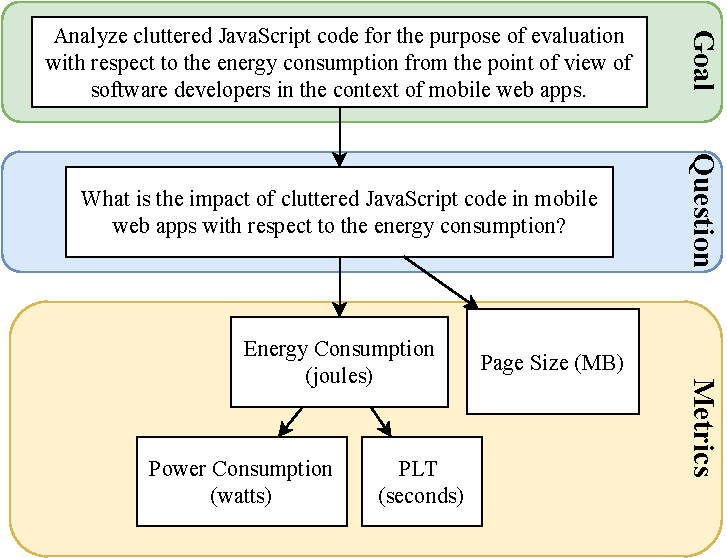
\includegraphics[width=8cm]{reportTemplate/figures/GQM.pdf}
\centering
\caption{The GQM Tree} \label{fig:gqm}
\end{figure}

Figure \ref{fig:gqm} presents a visual representation of the GQM. It hierarchically shows how the goal is obtained using the research question, and how the research question is answered using the metrics.
%\textcolor{red}{Page limit: 2}